



\chapter{Outliers}

Data are not perfect. At times, we run into the problem of one case having more influence over the least squares line than other cases. In regression, we assume that each case exerts equal influence on the regression line. In some cases, a single extreme value of a predictor can change the entire regression line. For example, consider Figure~\ref{fig:xout}. The graph on the left is for well behaving data, and the graph on the right shows the effect of a single extreme $x$ variable. Things are not as bad if we have an extreme value on the outcome, however, as we see in Figure~\ref{fig:yout}.

\begin{figure}
   \centering
   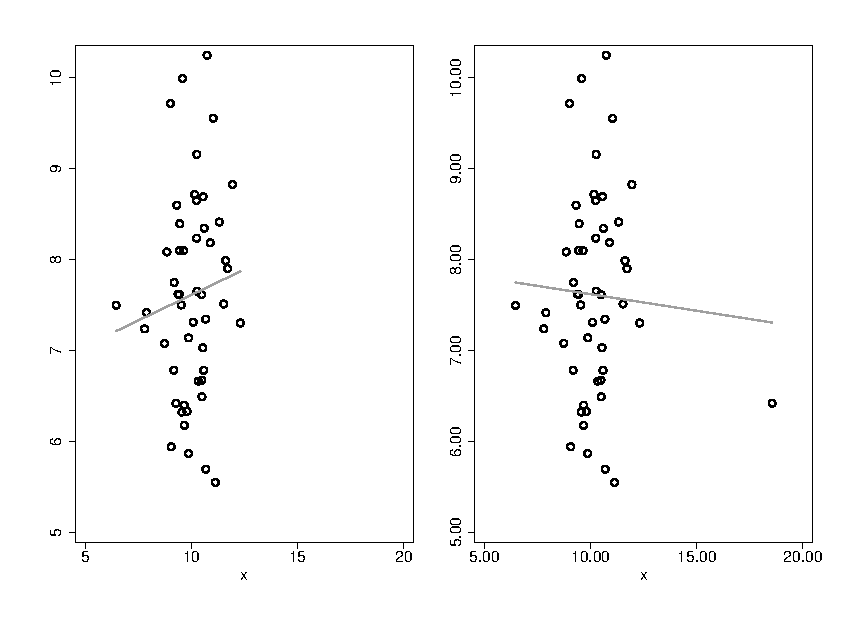
\includegraphics[angle=0,
           width=.75\textwidth]{xout.eps}
   \caption{Effect of extreme value of $x$}
  \label{fig:xout}
\end{figure}

\begin{figure}
   \centering
   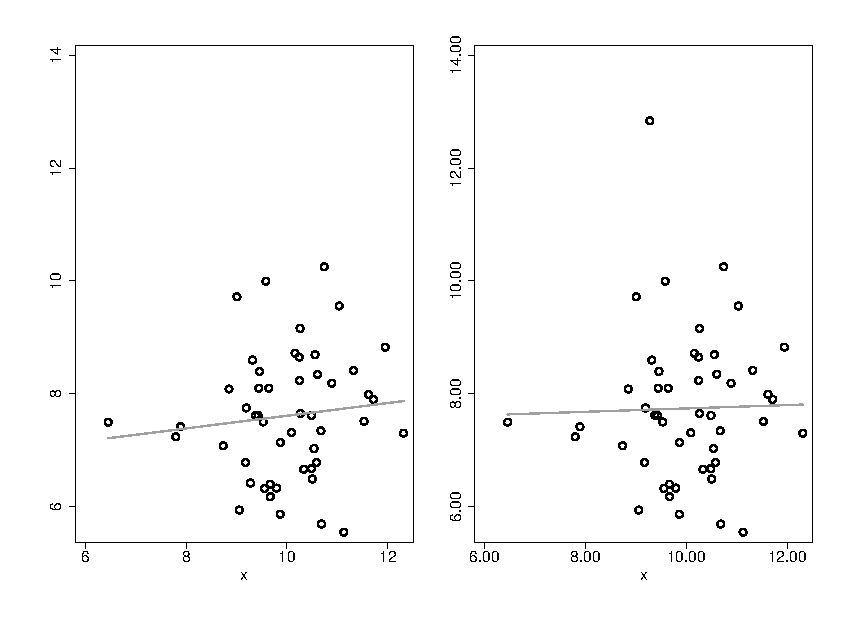
\includegraphics[angle=0,
           width=.75\textwidth]{yout.eps}
   \caption{Effect of extreme value of $y$}
  \label{fig:yout}
\end{figure}

Life isn’t so clear as these figures, however. How would be able to detect outlier variables when the number of cases are several hundred? Turns out there are a several different measures and tea-leaves to read. Let’s go over the favorites.

After you fit a model, there are about 6 big methods to detect outliers. These methods create a value for each case, and so these must be plotted for visual inspection. Generally by the case number, or "index."

As a reference, each measure plotted on normal data is displayed in Figure~\ref{fig:outnorm}.

\begin{figure}
   \centering
   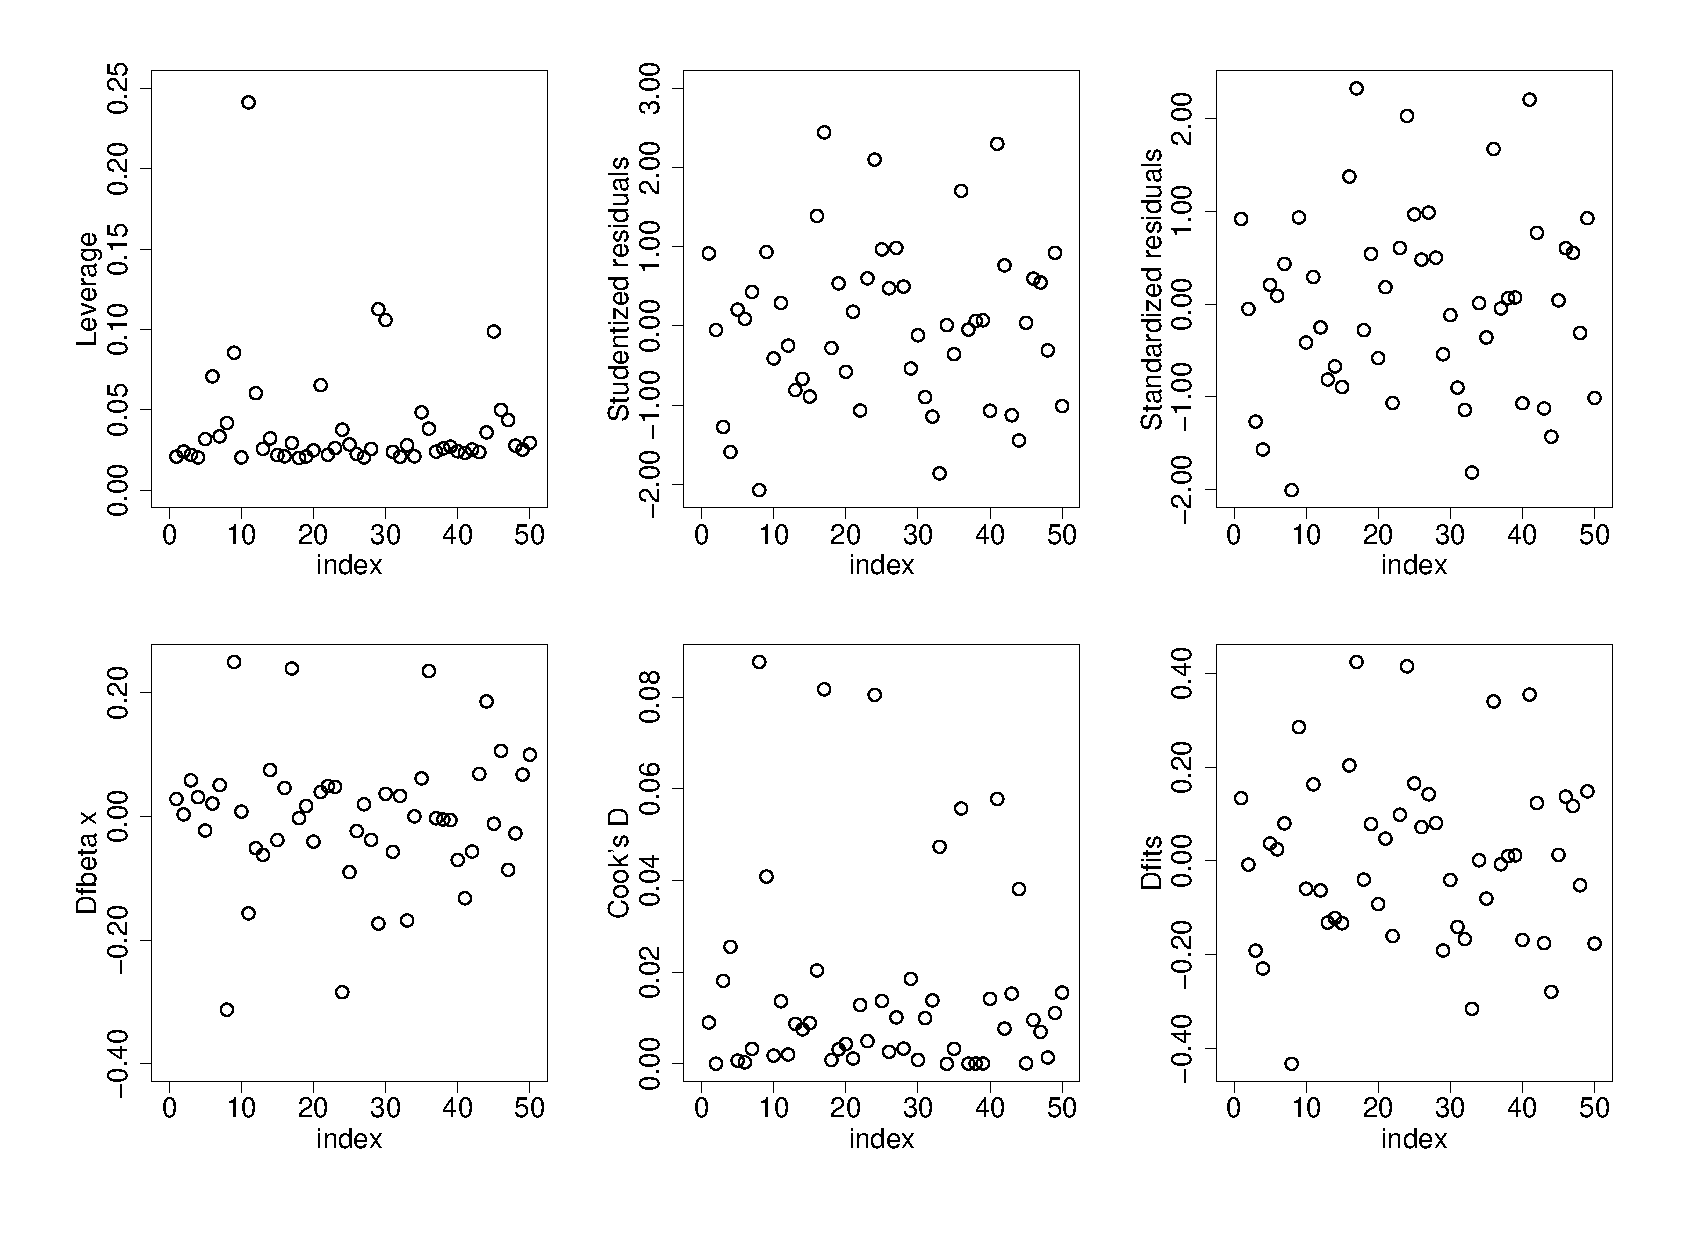
\includegraphics[angle=0,
           width=.75\textwidth]{normal_allmeasures_index.eps}
   \caption{Outlier values by case number of typical data in Table~\ref{tab:outdata}}
  \label{fig:outnorm}
\end{figure}

\section{Leverage}

If we examine the plots above, we can notice that outlier $x$ tend to drag the regression line around. This is called leverage. Leverage can be modeled by saying that each $j^{th}$ {\it fitted} value is a function of all the {\it observed} values of $y$,
\begin{equation}
\hat{y}_j=h_{1j}y_1+\ldots+h_{nj}y_n
\end{equation}
\begin{equation}
=\sum_{i=1}^N h_{ij}y_i
\end{equation}
In a simple bivariate regression, $h_j$ can be calculated with
\begin{equation}
h_j=\frac{1}{N}+\frac{\left(x_j-\bar{x}\right)^2}{\sum_{i=1}^N\left(x_i-\bar{x}\right)^2}
\end{equation}
For example, the calculations are shown in Table~\ref{tab:lever} for a small set of 5 cases.

\begin{table}[htbp]\centering
\caption{Example leverage calculations
\label{tab:lever}}
\begin{tabular}{lccc}
\hline
& $x$ & $\left(x-\bar{x}\right)^2$ & $h$ \\
\hline
&-0.960&0.006&0.201 \\
&-0.260&0.605&0.312 \\
&-3.020&3.928&0.930 \\
&-0.150&0.789&0.346 \\
&-0.800&0.057&0.211 \\
\hline
Sum & & 5.385 \\
Mean & -1.038 \\
\hline
\end{tabular}
\end{table}

If we examine the data in Table~\ref{tab:outdata} and plot the leverage values for the regression of $y$ on the $x$ column with the extreme case, you can see that case has a leverage value of 0.62 in Figure~ref{fig:xleverlab}.


\begin{figure}
   \centering
   \includegraphics[angle=0,
           width=.75\textwidth]{xout_hatvalues_label.eps}
   \caption{Scatter plot of data in Table~\ref{tab:outdata} ($y$ with extreme $x$) leverage values}
  \label{fig:xleverlab}
\end{figure}

However, a more useful method to detect which case(s) has (have) the extreme values is to plot the leverage value by case number, or {\it: index} as in Figure~\ref{fig:xlever}.

\begin{figure}
   \centering
   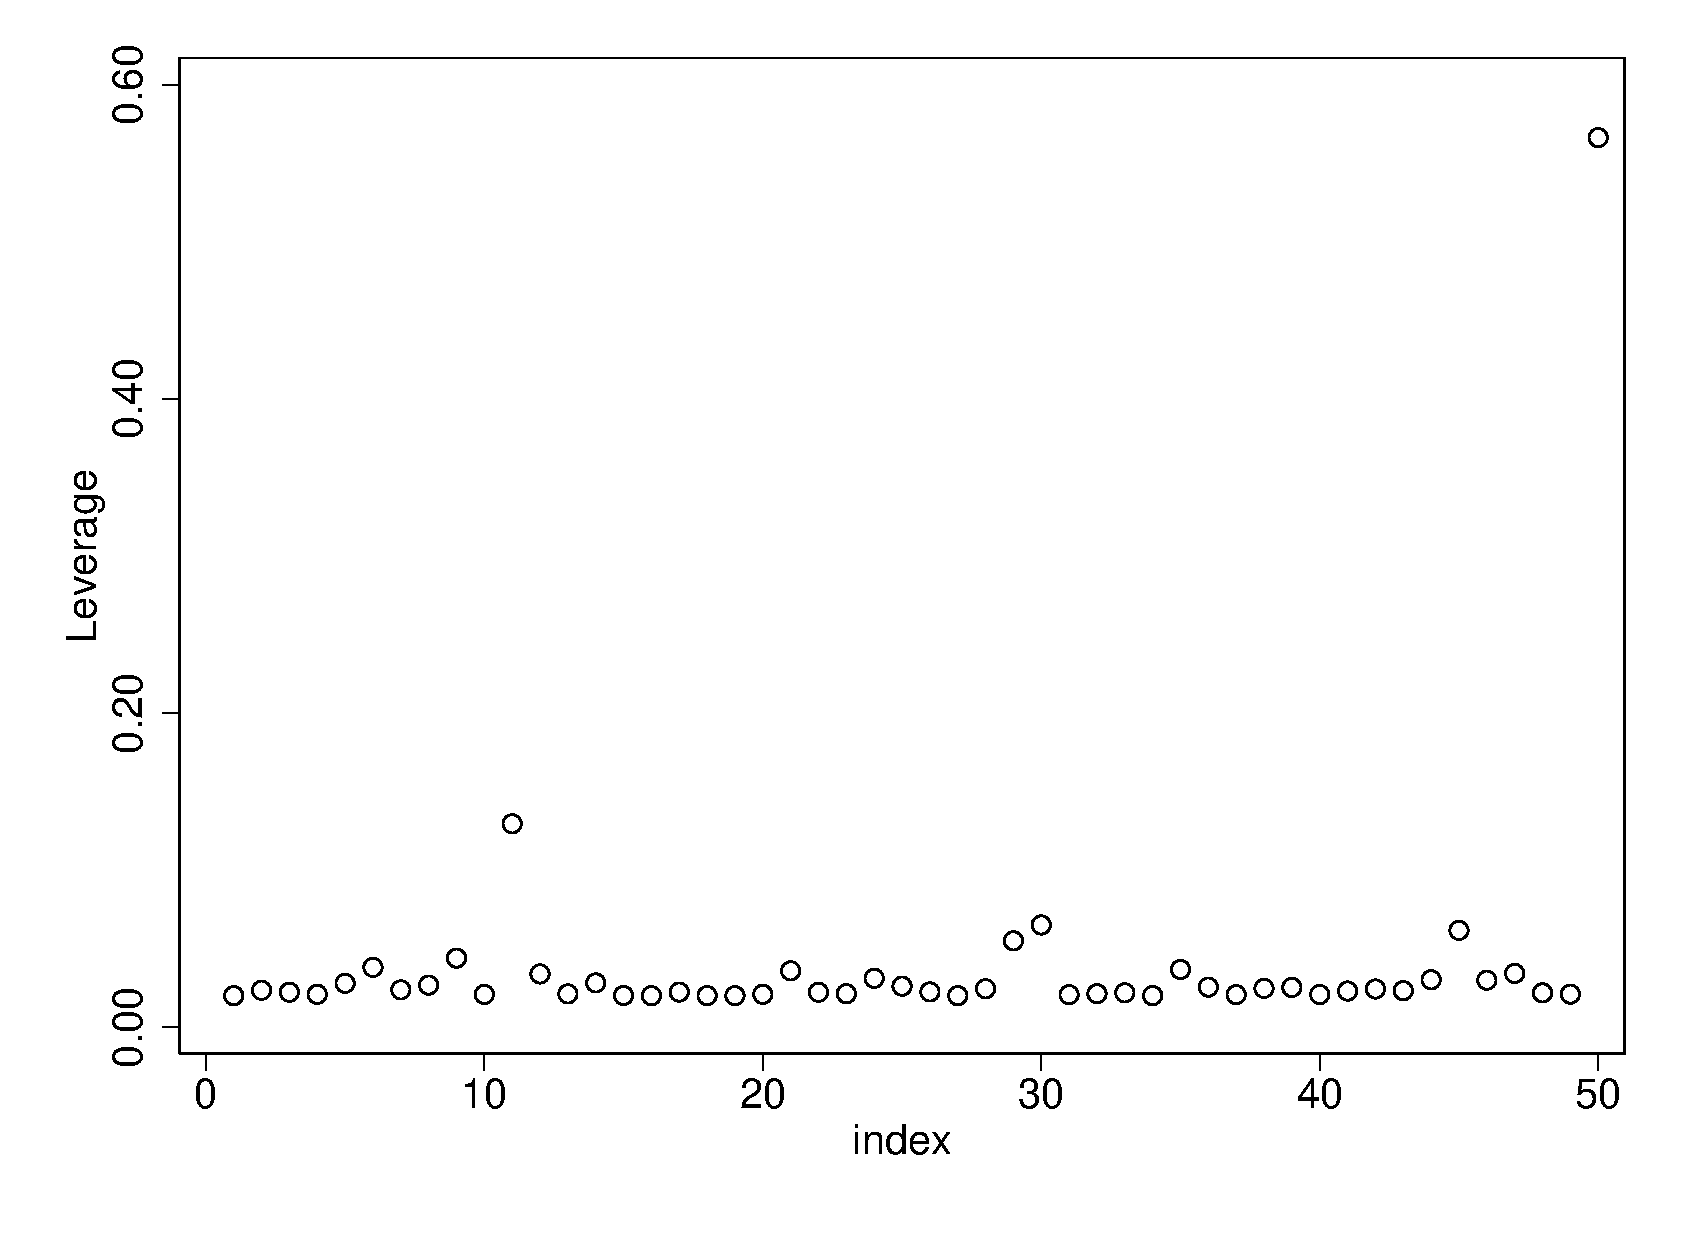
\includegraphics[angle=0,
           width=.75\textwidth]{xout_hatvalues_index.eps}
   \caption{Leverage values for extreme value of $x$ by case number of data in Table~\ref{tab:outdata}}
  \label{fig:xlever}
\end{figure}

As you can see in Figure~\ref{fig:ylever}, the leverage formulas have less utility in the cases of extreme $y$ values.

\begin{figure}
   \centering
   \includegraphics[angle=0,
           width=.75\textwidth]{yout_hatvalues_index.eps}
   \caption{Leverage values for extreme value of $y$ by case number of data in Table~\ref{tab:outdata}}
  \label{fig:ylever}
\end{figure}

\section{Standardized residuals}

Another plausible measure is the standardized residual from the model relative to the leverage, $h_i$

\begin{equation}
e^{\left(standardized\right)}_i=\frac{e_i}{s_e\sqrt{1-h_i}}
\end{equation}

where $s_e$ is the standard deviation of the residuals from the model. Figures with extraordinary values of $x$ and $y$ are displayed in Figures~\ref{fig:xstandard} and ~\ref{fig:ystandard}, respectively.

\begin{figure}
   \centering
   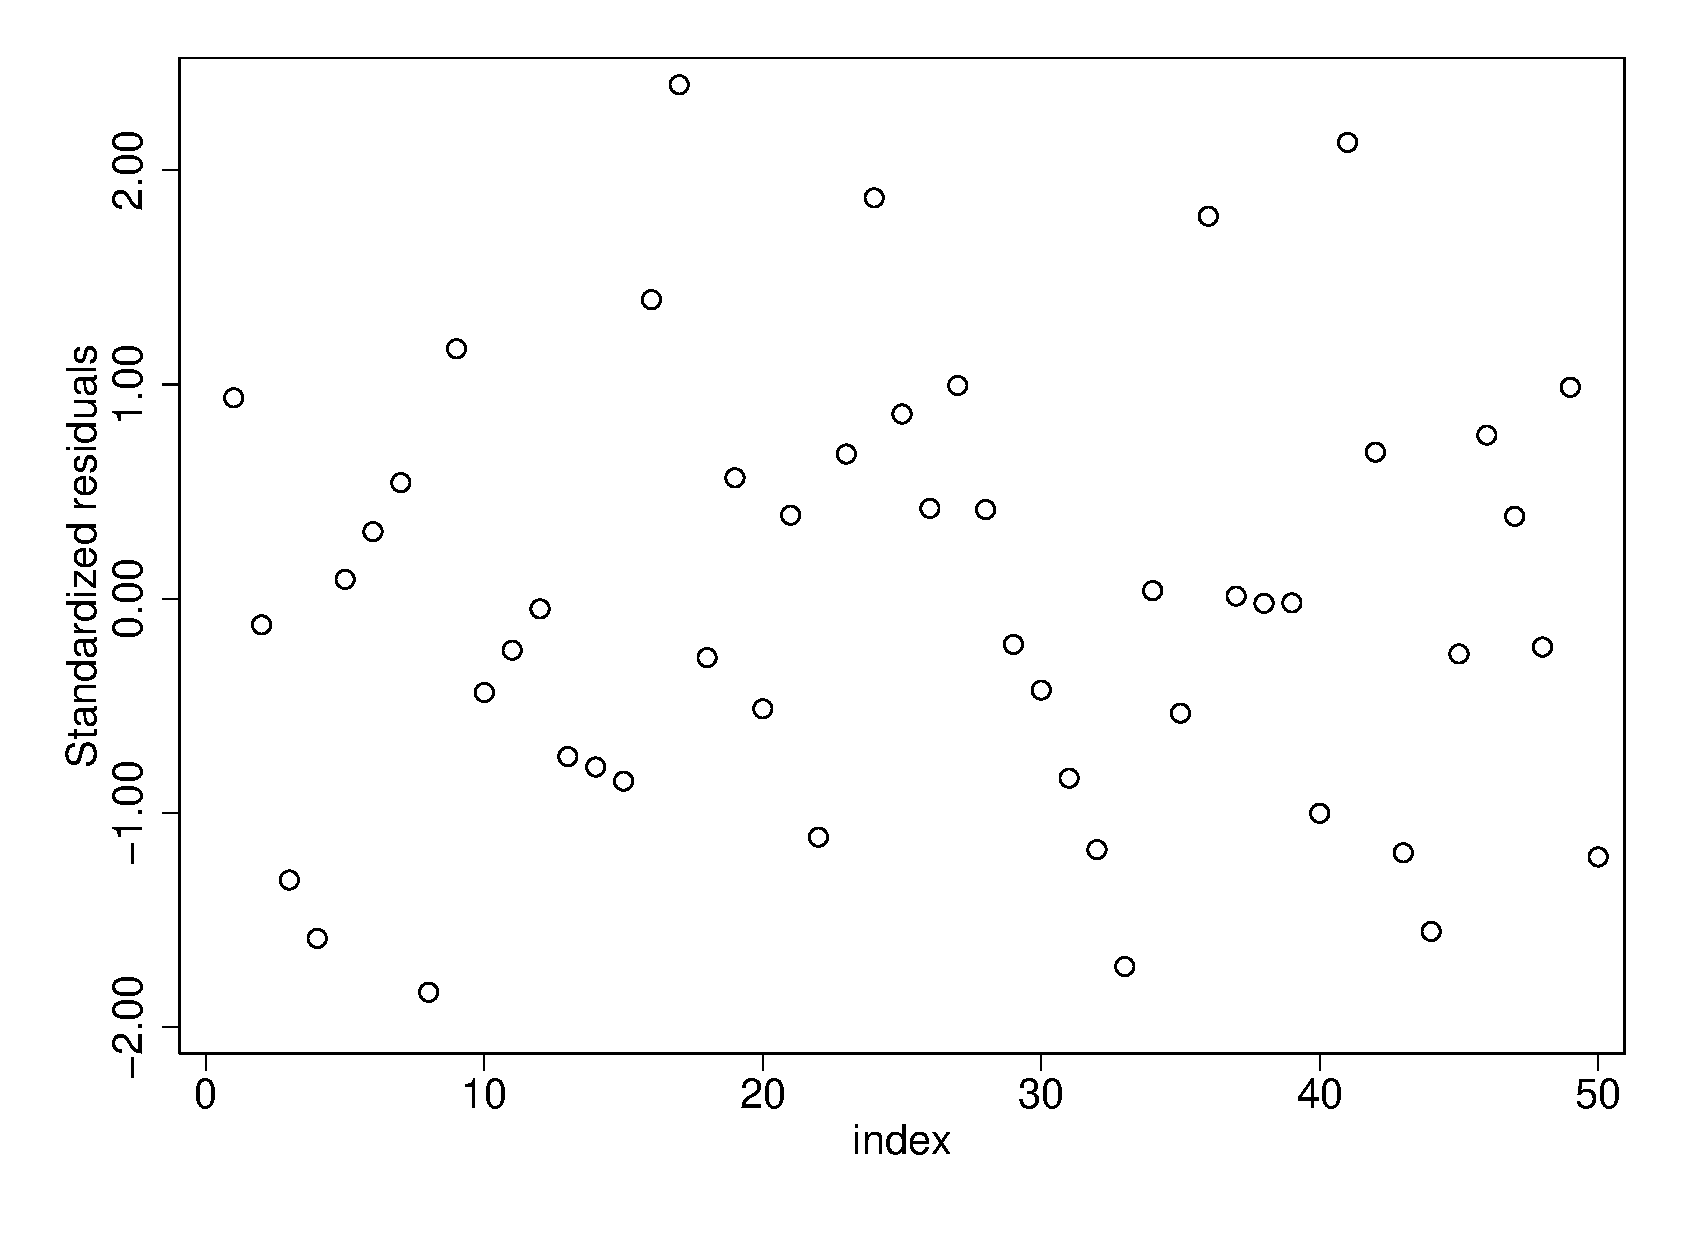
\includegraphics[angle=0,
           width=.75\textwidth]{xout_standard_index.eps}
   \caption{Standardized residual values for extreme value of $x$ by case number of data in Table~\ref{tab:outdata}}
  \label{fig:xstandard}
\end{figure}

\begin{figure}
   \centering
   \includegraphics[angle=0,
           width=.75\textwidth]{yout_standard_index.eps}
   \caption{Standardized residual values for extreme value of $y$ by case number of data in Table~\ref{tab:outdata}}
  \label{fig:ystandard}
\end{figure}

\section{Studentized residuals}

Another approach to residuals is to employ a standard deviation of the results from a model that excludes a particular case. Thus, for a given case $i$, this residual is
\begin{equation}
e^{\left(studentized\right)}_i=\frac{e_i}{s^{\left(-i\right)}_e\sqrt{1-h_i}}
\end{equation}
Figures with extraordinary values of $x$ and $y$ are displayed in Figures~\ref{fig:xstudent} and ~\ref{fig:ystudent}, respectively.
\begin{figure}
   \centering
   \includegraphics[angle=0,
           width=.75\textwidth]{xout_student_index.eps}
   \caption{Studentized residual values for extreme value of $x$ by case number of data in Table~\ref{tab:outdata}}
  \label{fig:xstudent}
\end{figure}

\begin{figure}
   \centering
   \includegraphics[angle=0,
           width=.75\textwidth]{yout_student_index.eps}
   \caption{Studentized residual values for extreme value of $y$ by case number of data in Table~\ref{tab:outdata}}
  \label{fig:ystudent}
\end{figure}


\section{DFBETA}

Yet another way to think about outliers is not how they influence the errors, but instead how they influence the regression slopes.
Thus, the DFBETA. This is the difference in a regression slope for predictor $p$ if a particular case $i$ was removed
\begin{equation}
D_{pi}=\beta_p - \beta_p^{-i}
\end{equation}

\begin{figure}
   \centering
   \includegraphics[angle=0,
           width=.75\textwidth]{xout_dfb_index.eps}
   \caption{Df-Beta values for extreme value of $x$ by case number of data in Table~\ref{tab:outdata}}
  \label{fig:xdfb}
\end{figure}

\begin{figure}
   \centering
   \includegraphics[angle=0,
           width=.75\textwidth]{yout_dfb_index.eps}
   \caption{Df-Beta values for extreme value of $y$ by case number of data in Table~\ref{tab:outdata}}
  \label{fig:ydfb}
\end{figure}

Figures with extraordinary values of $x$ and $y$ are displayed in Figures~\ref{fig:xdfb} and ~\ref{fig:ydfb}, respectively.

\section{Cook's distance}

The Cook's distance measure combines the leverage values with standardized residuals
\begin{equation}
D_i = \frac{e^{\left(standardized\right)}_i}{k+1}\times\frac{h_i}{1-h_i}
\end{equation}


\begin{figure}
   \centering
   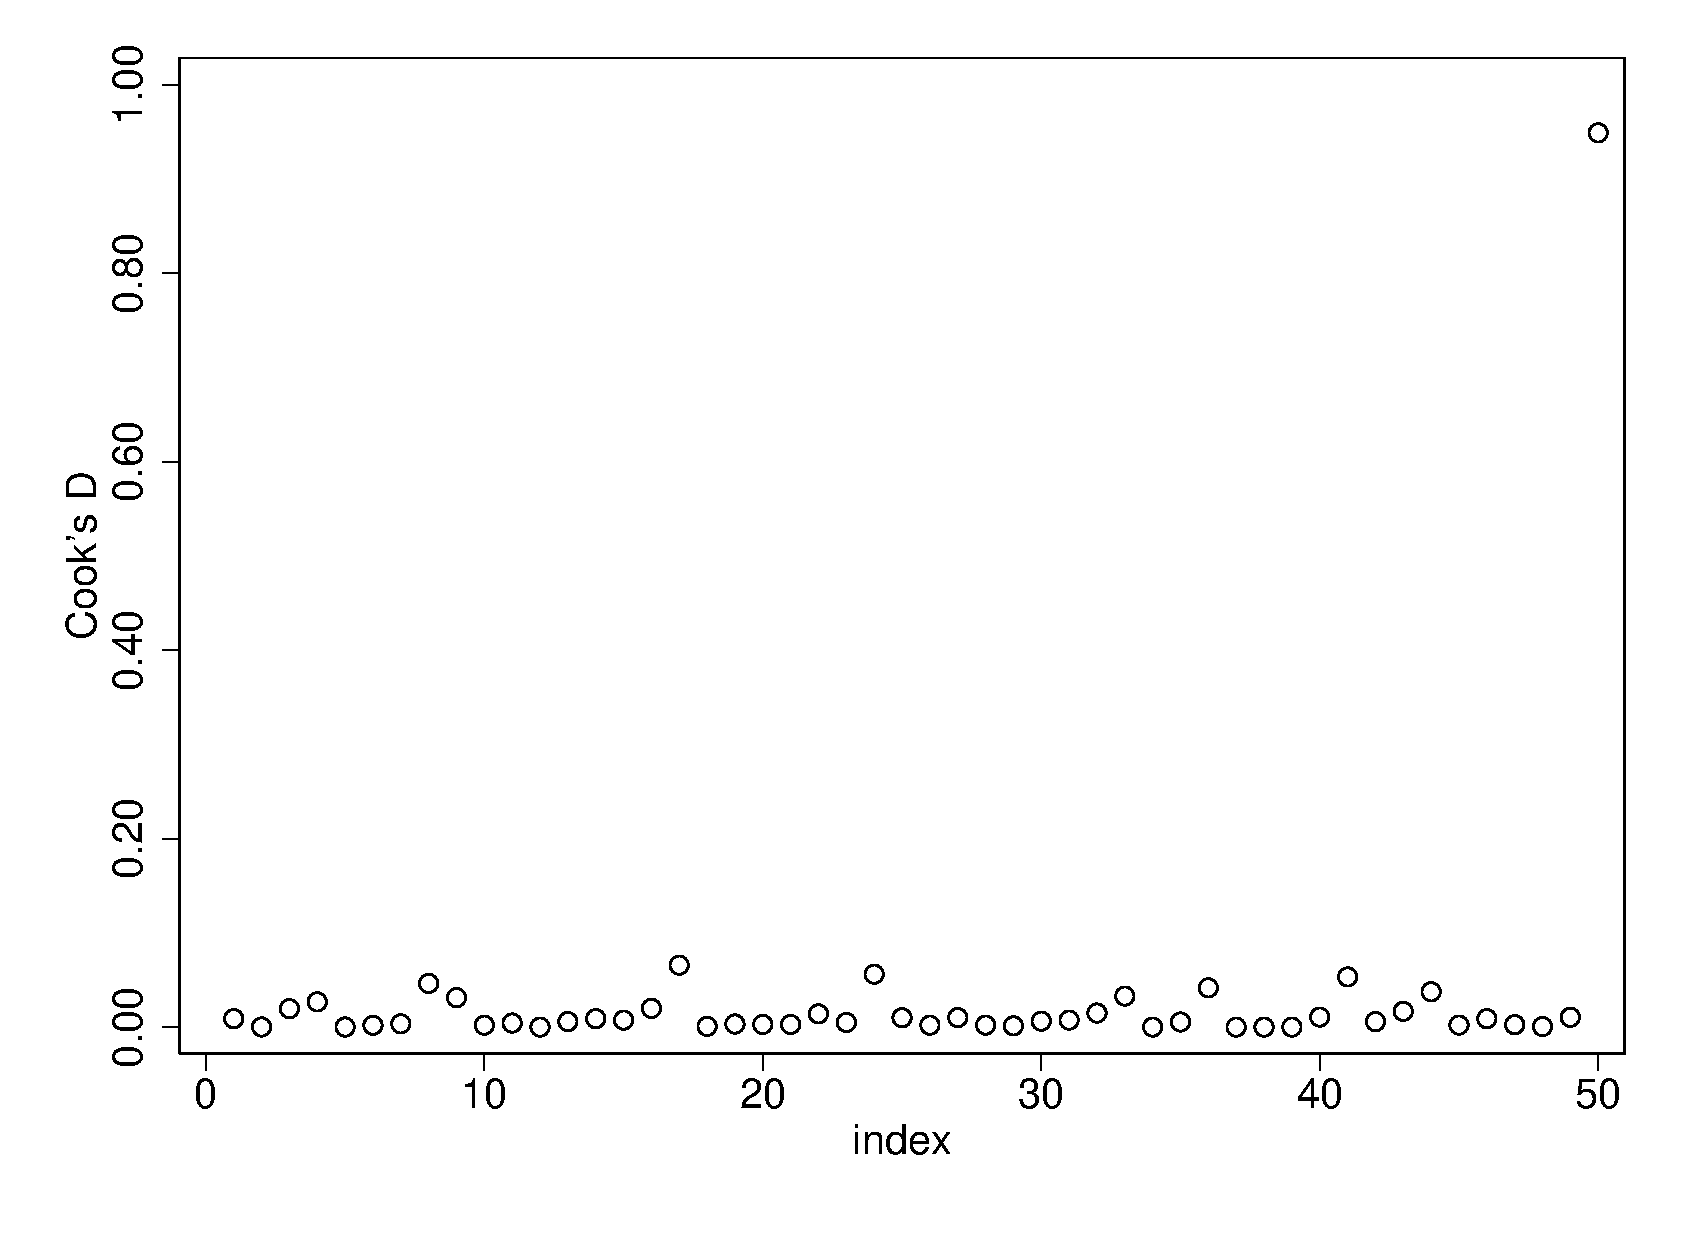
\includegraphics[angle=0,
           width=.75\textwidth]{xout_cooks_index.eps}
   \caption{Cook's distance values for extreme value of $x$ by case number of data in Table~\ref{tab:outdata}}
  \label{fig:xcook}
\end{figure}

\begin{figure}
   \centering
   \includegraphics[angle=0,
           width=.75\textwidth]{yout_cooks_index.eps}
   \caption{Cook's distance values for extreme value of $y$ by case number of data in Table~\ref{tab:outdata}}
  \label{fig:ycook}
\end{figure}

Figures with extraordinary values of $x$ and $y$ are displayed in Figures~\ref{fig:xcook} and ~\ref{fig:ycook}, respectively.

\section{Dfits}


Similar to Cook's distance is the DFITS measure.

\begin{equation}
D_i = e_i\times \sqrt{\frac{h_i}{1-h_i}}
\end{equation}

Figures with extraordinary values of $x$ and $y$ are displayed in Figures~\ref{fig:xdfit} and ~\ref{fig:ydfit}, respectively.

\begin{figure}
   \centering
   \includegraphics[angle=0,
           width=.75\textwidth]{xout_dfit_index.eps}
   \caption{D-fit values for extreme value of $x$ by case number of data in Table~\ref{tab:outdata}}
  \label{fig:xdfit}
\end{figure}

\begin{figure}
   \centering
   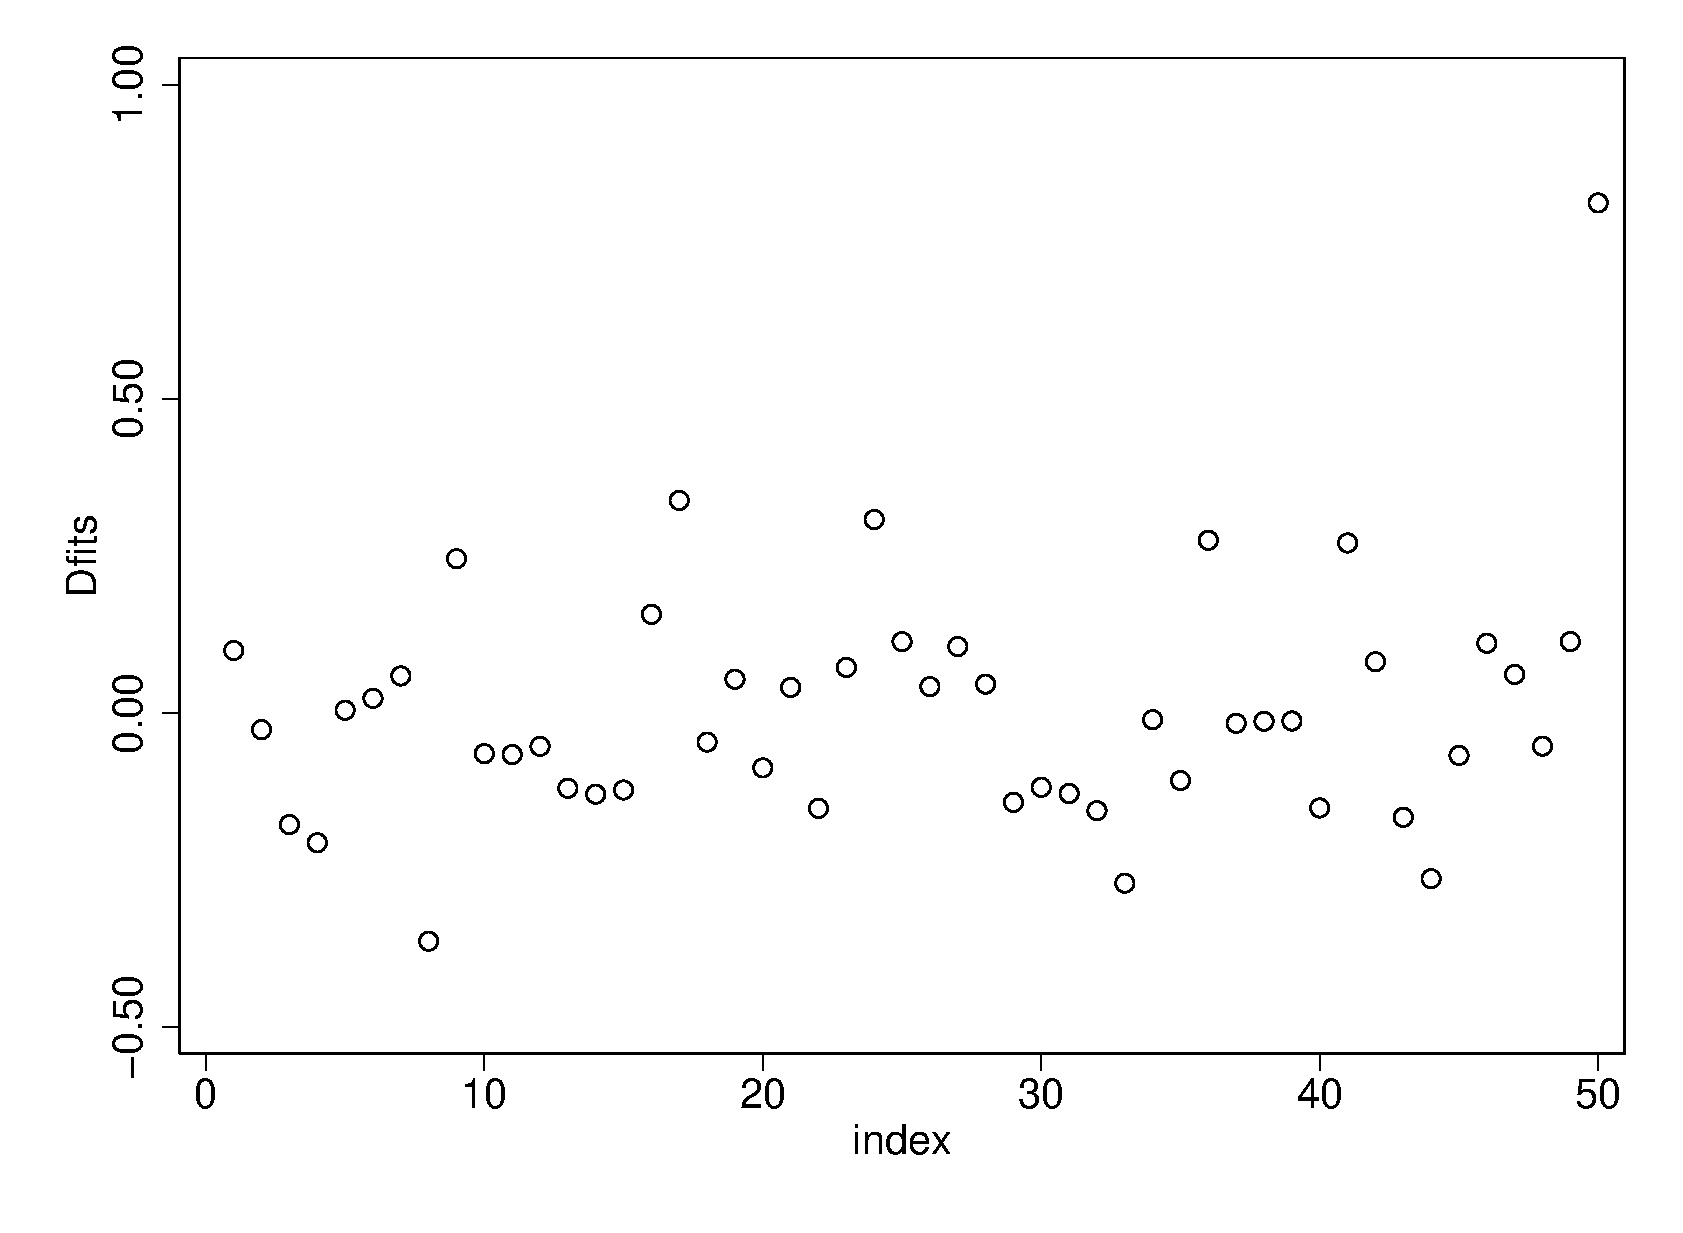
\includegraphics[angle=0,
           width=.75\textwidth]{yout_dfit_index.eps}
   \caption{D-fit values for extreme value of $y$ by case number of data in Table~\ref{tab:outdata}}
  \label{fig:ydfit}
\end{figure}

\section{Summary}

As you can see, there are several measures to detect outliers. In most cases, it will be difficult to spot them initially. Table~\ref{tab:outsum} gives a general summary of the different methods and how well they work to discover extreme $x$ or $y$ values. In the end, I recommend the use of the Dfits measure as it combines the leverage values with the residuals (thus involves both the outcome and predictors).

\begin{table}[htbp]\centering
\caption{Summary of outlier measures for extreme $x$ and $y$
\label{tab:outsum}}
\begin{tabular}{lll}
\hline
Measure & Extreme $x$ & Extreme $y$ \\
\hline
Leverage & Yes & No \\
Standardized residuals & No & Yes \\
Studentized residuals & Maybe & Yes \\
DFBETA & Yes & No \\
Cook's distance & Yes & Maybe \\
DFits & Yes & Yes \\
\hline
\end{tabular}
\end{table}